\chapter{Latex錯誤修正}
在製作latex報告中,經常會出現錯誤,在不懂錯誤的情況下,詢問chatGPT尋求解答
\begin{figure}[ht]
  \begin{minipage}{0.5\textwidth}
    \centering
    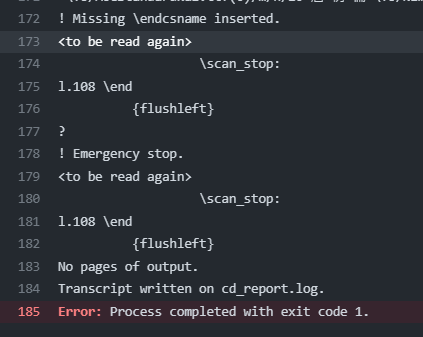
\includegraphics[width=\textwidth]{beginend錯誤}
    \caption{beginend錯誤}
  \end{minipage}%
  \begin{minipage}{0.5\textwidth}
    \centering
    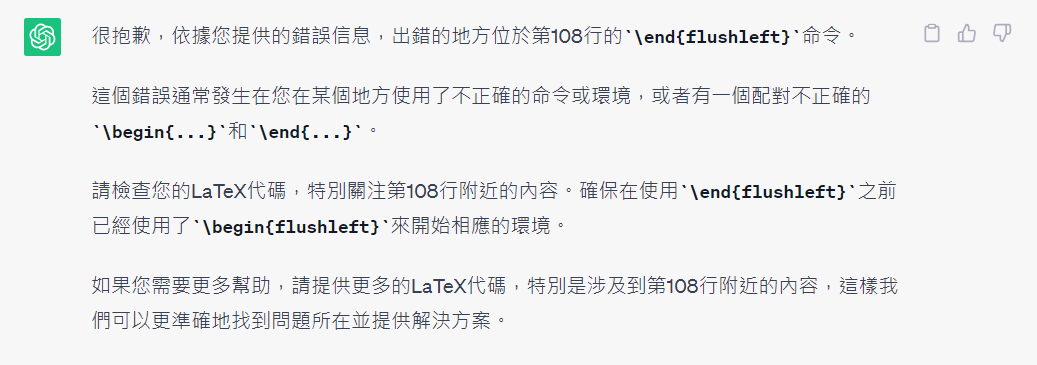
\includegraphics[width=\textwidth]{beginend錯誤解答}
    \caption{beginend錯誤解答}
  \end{minipage}
\end{figure}
此情況可能為begin跟end數量不對等造成的錯誤。\\
\begin{figure}[ht]
  \begin{minipage}{0.5\textwidth}
    \centering
    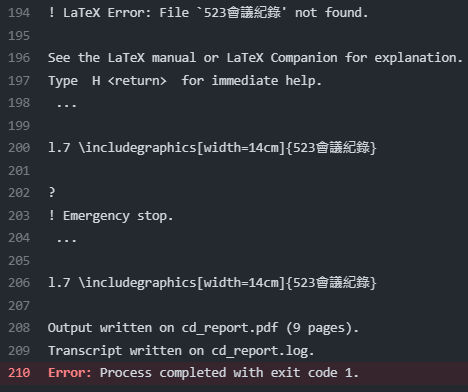
\includegraphics[width=\textwidth]{圖片名打錯}
    \caption{圖片名打錯}
  \end{minipage}%
  \begin{minipage}{0.5\textwidth}
    \centering
    
\includegraphics[width=\textwidth]{圖片名打錯解答}
    \caption{圖片名打錯解答}
  \end{minipage}
\end{figure}
在[width]後面接的是image裡面的圖檔名稱,要在目錄中顯示的名稱要打在caption後面。\\

\begin{figure}[ht]
  \begin{minipage}{0.5\textwidth}
    \centering
    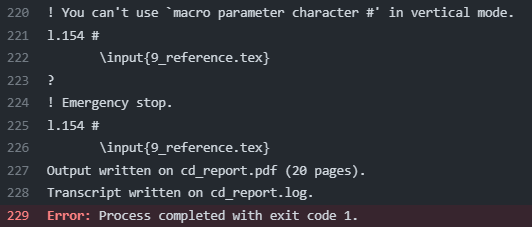
\includegraphics[width=\textwidth]{符號打錯}
    \caption{符號打錯}
  \end{minipage}%
  \begin{minipage}{0.5\textwidth}
    \centering
    
\includegraphics[width=\textwidth]{符號打錯解答}
    \caption{符號打錯解答}
  \end{minipage}
\end{figure}
在latex程式碼中,想要屏蔽不想要出現的內容,不能打#,要在該段最前面輸入%。\\

\begin{figure}[ht]
  \begin{minipage}{0.5\textwidth}
    \centering
    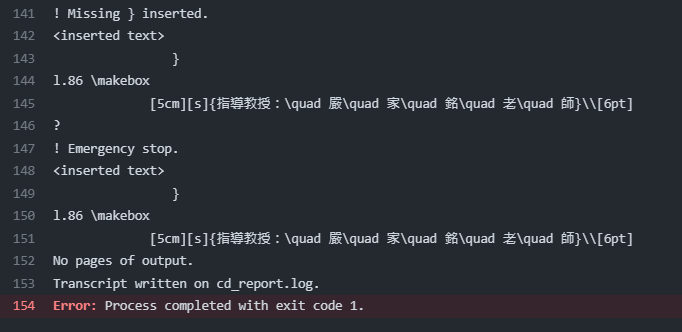
\includegraphics[width=\textwidth]{缺少符號}
    \caption{缺少符號}
  \end{minipage}%
  \begin{minipage}{0.5\textwidth}
    \centering
    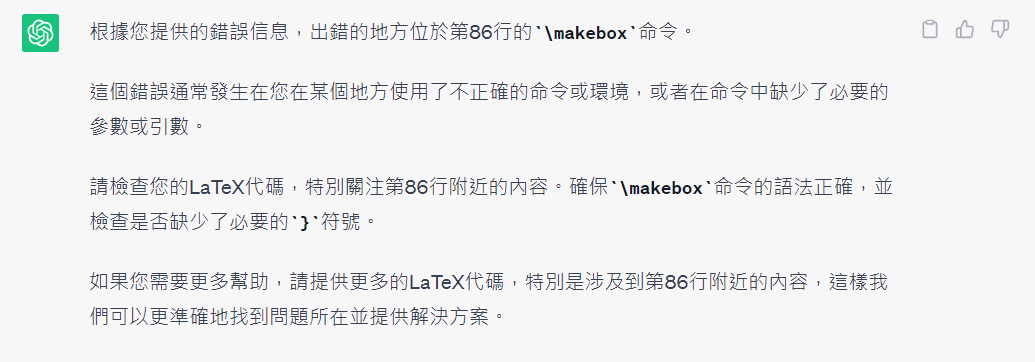
\includegraphics[width=\textwidth]{缺少符號解答}
    \caption{缺少符號解答}
  \end{minipage}
\end{figure}
要注意是否都有輸入正確的符號,括號要對稱。//

\begin{figure}[ht]
  \begin{minipage}{0.5\textwidth}
    \centering
    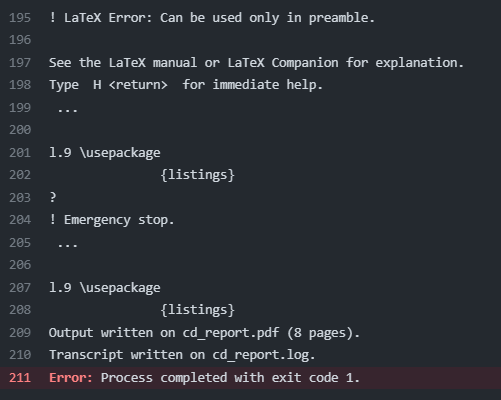
\includegraphics[width=\textwidth]{設定錯誤}
    \caption{設定錯誤}
  \end{minipage}%
  \begin{minipage}{0.5\textwidth}
    \centering
    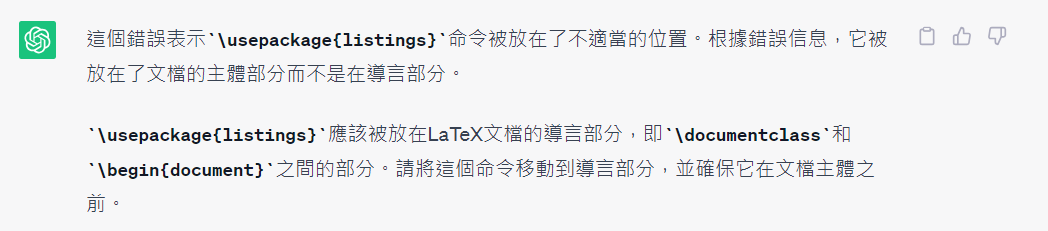
\includegraphics[width=\textwidth]{設定錯誤解答}
    \caption{設定錯誤解答}
  \end{minipage}
\end{figure}
設定文章內容的條件應該要放在最前頁,不能放在篇章中。
\newpage
